% Options for packages loaded elsewhere
\PassOptionsToPackage{unicode}{hyperref}
\PassOptionsToPackage{hyphens}{url}
%
\documentclass[
  ignorenonframetext,
]{beamer}
\title{A mechanistic model for superspreading}
\author{Suzanne O'Regan}
\date{Drake Lab Meeting, 11/12/2021}

\usepackage{pgfpages}
\setbeamertemplate{caption}[numbered]
\setbeamertemplate{caption label separator}{: }
\setbeamercolor{caption name}{fg=normal text.fg}
\beamertemplatenavigationsymbolsempty
% Prevent slide breaks in the middle of a paragraph
\widowpenalties 1 10000
\raggedbottom
\setbeamertemplate{part page}{
  \centering
  \begin{beamercolorbox}[sep=16pt,center]{part title}
    \usebeamerfont{part title}\insertpart\par
  \end{beamercolorbox}
}
\setbeamertemplate{section page}{
  \centering
  \begin{beamercolorbox}[sep=12pt,center]{part title}
    \usebeamerfont{section title}\insertsection\par
  \end{beamercolorbox}
}
\setbeamertemplate{subsection page}{
  \centering
  \begin{beamercolorbox}[sep=8pt,center]{part title}
    \usebeamerfont{subsection title}\insertsubsection\par
  \end{beamercolorbox}
}
\AtBeginPart{
  \frame{\partpage}
}
\AtBeginSection{
  \ifbibliography
  \else
    \frame{\sectionpage}
  \fi
}
\AtBeginSubsection{
  \frame{\subsectionpage}
}
\usepackage{amsmath,amssymb}
\usepackage{lmodern}
\usepackage{iftex}
\ifPDFTeX
  \usepackage[T1]{fontenc}
  \usepackage[utf8]{inputenc}
  \usepackage{textcomp} % provide euro and other symbols
\else % if luatex or xetex
  \usepackage{unicode-math}
  \defaultfontfeatures{Scale=MatchLowercase}
  \defaultfontfeatures[\rmfamily]{Ligatures=TeX,Scale=1}
\fi
% Use upquote if available, for straight quotes in verbatim environments
\IfFileExists{upquote.sty}{\usepackage{upquote}}{}
\IfFileExists{microtype.sty}{% use microtype if available
  \usepackage[]{microtype}
  \UseMicrotypeSet[protrusion]{basicmath} % disable protrusion for tt fonts
}{}
\makeatletter
\@ifundefined{KOMAClassName}{% if non-KOMA class
  \IfFileExists{parskip.sty}{%
    \usepackage{parskip}
  }{% else
    \setlength{\parindent}{0pt}
    \setlength{\parskip}{6pt plus 2pt minus 1pt}}
}{% if KOMA class
  \KOMAoptions{parskip=half}}
\makeatother
\usepackage{xcolor}
\IfFileExists{xurl.sty}{\usepackage{xurl}}{} % add URL line breaks if available
\IfFileExists{bookmark.sty}{\usepackage{bookmark}}{\usepackage{hyperref}}
\hypersetup{
  pdftitle={A mechanistic model for superspreading},
  pdfauthor={Suzanne O'Regan},
  hidelinks,
  pdfcreator={LaTeX via pandoc}}
\urlstyle{same} % disable monospaced font for URLs
\newif\ifbibliography
\usepackage{graphicx}
\makeatletter
\def\maxwidth{\ifdim\Gin@nat@width>\linewidth\linewidth\else\Gin@nat@width\fi}
\def\maxheight{\ifdim\Gin@nat@height>\textheight\textheight\else\Gin@nat@height\fi}
\makeatother
% Scale images if necessary, so that they will not overflow the page
% margins by default, and it is still possible to overwrite the defaults
% using explicit options in \includegraphics[width, height, ...]{}
\setkeys{Gin}{width=\maxwidth,height=\maxheight,keepaspectratio}
% Set default figure placement to htbp
\makeatletter
\def\fps@figure{htbp}
\makeatother
\setlength{\emergencystretch}{3em} % prevent overfull lines
\providecommand{\tightlist}{%
  \setlength{\itemsep}{0pt}\setlength{\parskip}{0pt}}
\setcounter{secnumdepth}{-\maxdimen} % remove section numbering
\usepackage{amsmath}
\ifLuaTeX
  \usepackage{selnolig}  % disable illegal ligatures
\fi

\begin{document}
\frame{\titlepage}

\begin{frame}{Heterogeneity in disease transmission arises frequently in
epidemics}
\protect\hypertarget{heterogeneity-in-disease-transmission-arises-frequently-in-epidemics}{}
\begin{itemize}
\tightlist
\item
  Individuals can vary in their ability to transmit infectious agents
  through biological, behavioral and environmental factors
\item
  Superspreading events, where one infected individual gives rise to a
  large number of secondary infections in a single generation, may be
  the source of most of the secondary cases in a population
\item
  The first wave of the SARS CoV-2 pandemic was characterized by
  multiple superspreading events
\item
  Understanding the role of superspreading individuals in fuelling
  transmission in an outbreak is important for epidemic containment.
\item
  Superspreading often modeled using branching processes
\end{itemize}
\end{frame}

\begin{frame}{Modeling the number of secondary infections per infectious
individual using a branching process: assumptions}
\protect\hypertarget{modeling-the-number-of-secondary-infections-per-infectious-individual-using-a-branching-process-assumptions}{}
\begin{itemize}
\tightlist
\item
  Homogeneous population
\item
  Infectious individuals are independent from each other
\item
  Early in an epidemic when depletion of susceptibles can be ignored
\item
  Negative binomial model commonly used for superspreading
\item
  Negative binomial has two parameters: mean \(R_0\) and dispersion
  parameter \(k\)
\item
  Macro-level: discrete time, in units equal to the infectious period of
  an individual
\end{itemize}
\end{frame}

\begin{frame}{The negative binomial offspring distribution exhibits
hallmarks of transmission heterogeneity}
\protect\hypertarget{the-negative-binomial-offspring-distribution-exhibits-hallmarks-of-transmission-heterogeneity}{}
\begin{columns}[T]
\begin{column}{0.4\textwidth}
\begin{figure}
\centering
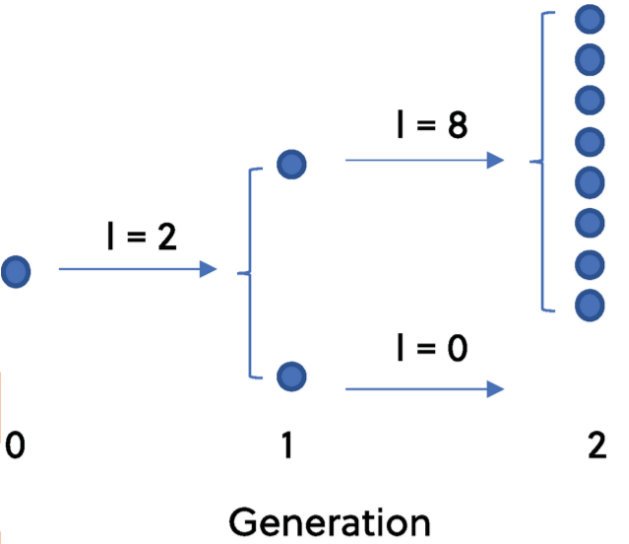
\includegraphics{Althouseetal2020BranchingProcess.png}
\caption{Negative binomial model. Source: Althouse et al.~2020}
\end{figure}
\end{column}

\begin{column}{0.6\textwidth}
\begin{itemize}
\item Greater variability in the number of secondary infections (fat tailed)
\item Smaller probability of major epidemics
\item Greater variability in chain sizes
\item Larger probability of observing no secondary infections and of observing small chains that go extinct
\end{itemize}
\end{column}
\end{columns}
\end{frame}

\begin{frame}{Discrete-time branching process embedded within continuous
time branching process}
\protect\hypertarget{discrete-time-branching-process-embedded-within-continuous-time-branching-process}{}
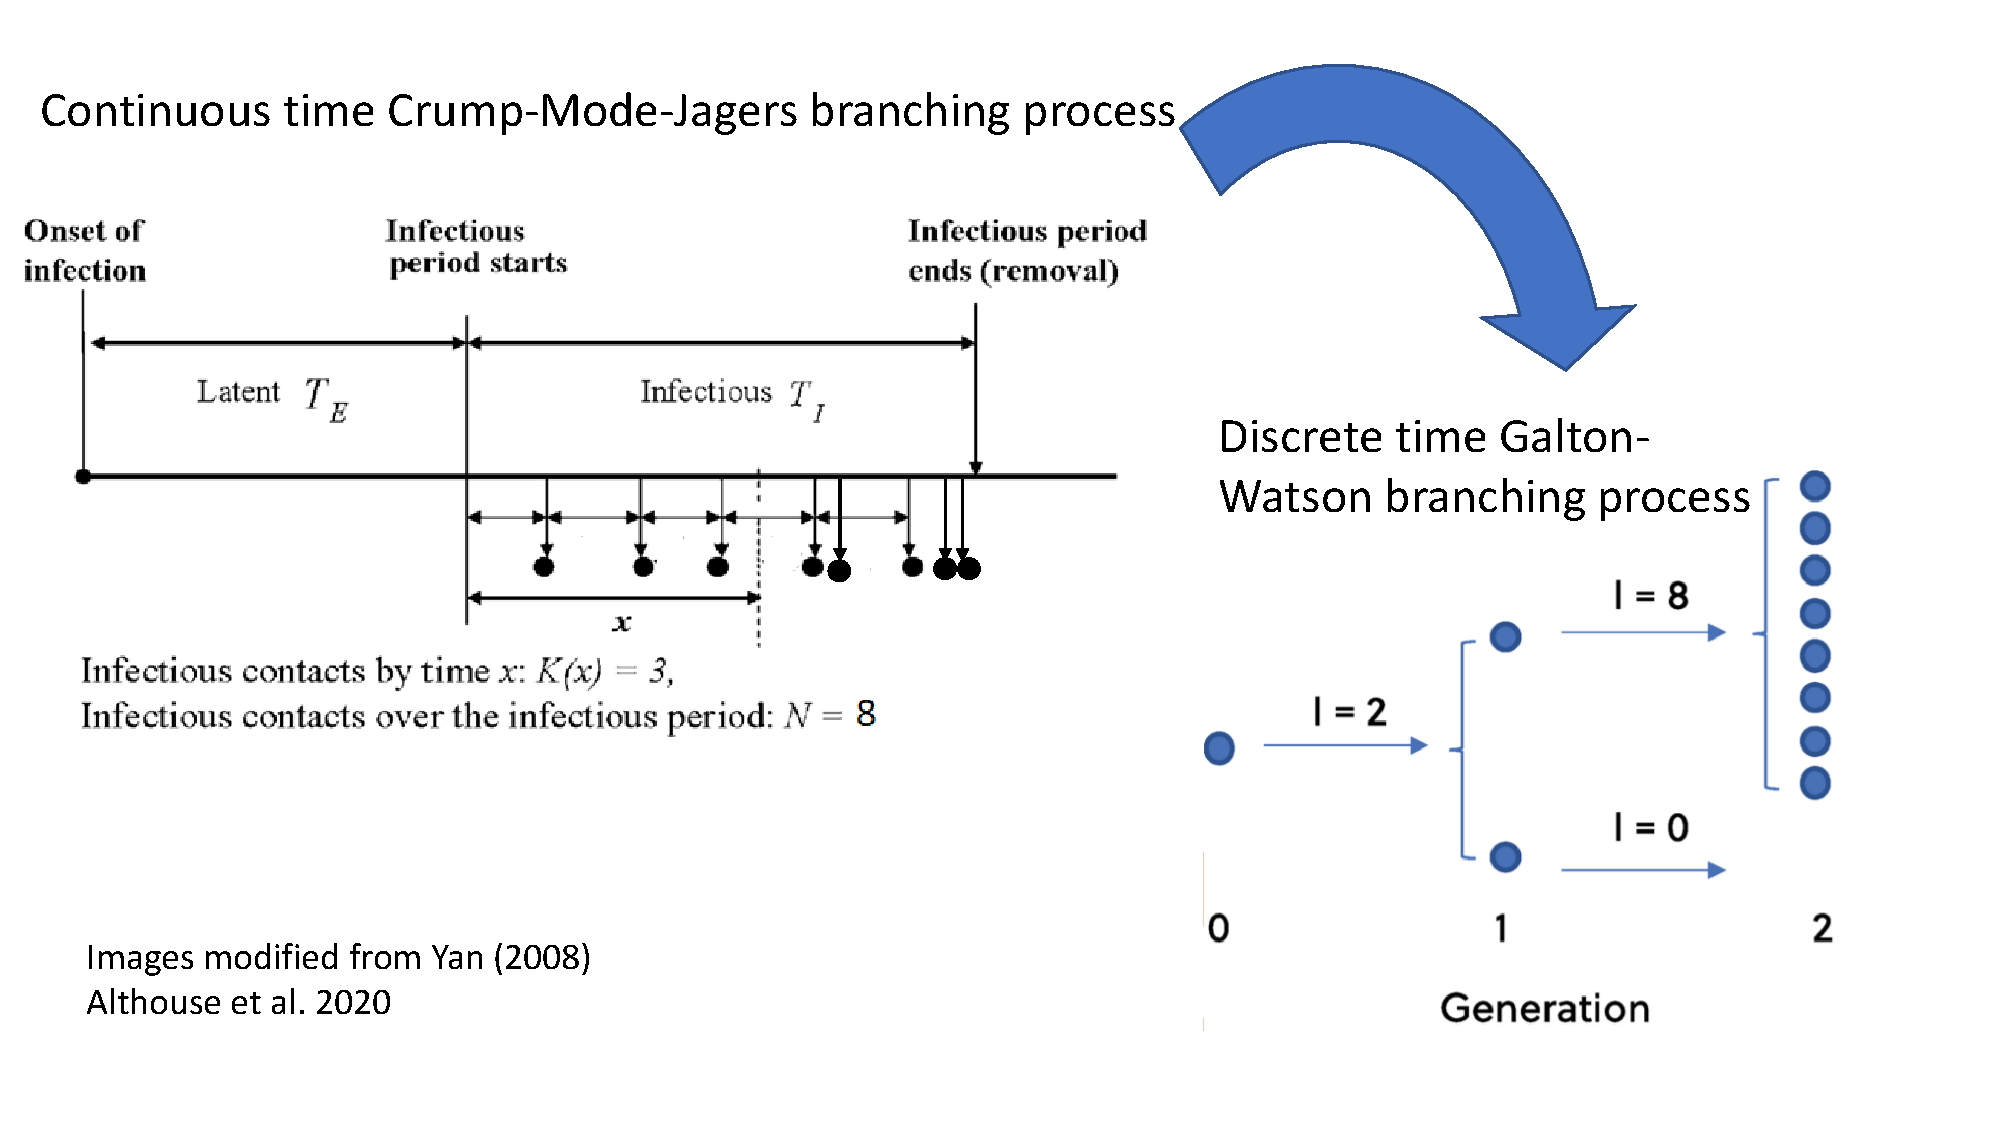
\includegraphics[width=1.1\textwidth,height=\textheight]{BranchingProcesses.pdf}
\end{frame}

\begin{frame}{}
\protect\hypertarget{section}{}
\begin{columns}[T]
\begin{column}{0.4\textwidth}
\begin{figure}
\centering
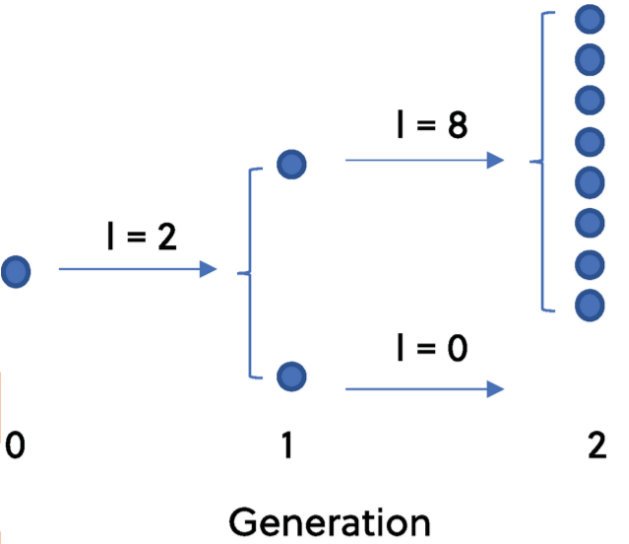
\includegraphics{Althouseetal2020BranchingProcess.png}
\caption{Negative binomial model. Source: Althouse et al.~2020}
\end{figure}
\end{column}

\begin{column}{0.6\textwidth}
\begin{itemize}
\tightlist
\item
  Typically researchers simulate the number of secondary infections per
  individual in discrete time using an offspring distribution arising
  from a GW process
\item
  Additionally, the theory of GW processes offers many analytical and
  computational advantages. The number of cases per generation can be
  simulated easily, the probability of a large outbreak can be
  calculated and the distribution of transmission chains that go extinct
  can often be obtained
\end{itemize}
\end{column}
\end{columns}
\end{frame}

\begin{frame}{Common model for superspreading: the negative binomial
model}
\protect\hypertarget{common-model-for-superspreading-the-negative-binomial-model}{}
\begin{itemize}
\item
  negative binomial model = Poisson-gamma mixture
\item
  discrete time (individual infectious period = generation)
\item
  \begin{enumerate}
  [a)]
  \tightlist
  \item
    Poisson contact process with intensity \(\lambda x\) with
    gamma-distributed infectious period \(x\) with mean \(1/\gamma\) and
    CV \(1/\sqrt{k}\) gives rise to negative binomial offspring
    distribution for the number of secondary infections per infectious
    individual over the course of their infectious period with mean
    \(R_0\) and dispersion parameter \(k\)
  \end{enumerate}
\item
  \begin{enumerate}
  [a)]
  \setcounter{enumi}{1}
  \tightlist
  \item
    Lloyd-Smith et al.~(2005) assumed individual reproductive number
    \(\nu\) is gamma-distributed and demographic stochasticity in
    individuals follows a Poisson process, yielding a negative binomial
    offspring distribution with mean \(R_0\) and dispersion parameter
    \(k\)
  \end{enumerate}
\item
  Limitation: The model does not take population risk structure into
  account. The population may be grouped by social, biological,
  behavioral or environmental factors
\end{itemize}
\end{frame}

\begin{frame}{Mechanisms for superspreading transmission}
\protect\hypertarget{mechanisms-for-superspreading-transmission}{}
\begin{table}\scriptsize
\begin{tabular}{ll}
\textbf{Source of heterogeneity} & \textbf{Factor} \\[3pt]
\textbf{Micro-level binary} &  \\[3pt]
Proximity to susceptible individuals (remote worker vs. healthcare worker) 
& Environmental \\
Transmission mode (e.g., aerosol vs. droplet transmission)   &Biological  \\
Symptomatology (e.g. shedding at high rates vs. low rates) &  Biological
\\
Compliance behaviors (e.g., self-isolation when sick vs. no self isolation)   &Behavioral \\
Vaccination status (i.e., vaccinated vs. not vaccinated) & Behavioral\\
Infectiousness (e.g., having underlying health conditions or not) & Biological or \\
& Behavioral \\[3pt]
\textbf{Micro-level continuous} &  \\[3pt]
Symptomatology (infectiousness affecting probability of infection) & Biological \\
 Symptomatology  (severe longlasting symptoms)& Biological \\ 
\end{tabular}
\end{table}

Models for the distribution of secondary infections that combine
heterogeneous transmission patterns with realistic distributions of
infection duration are needed
\end{frame}

\begin{frame}{Key questions}
\protect\hypertarget{key-questions}{}
\begin{itemize}
\tightlist
\item
  Does the mechanistic addition of population structure induce
  qualitatively different outbreak patterns from a standard
  superspreading model?
\item
  How does decreasing the level of superspreading by a) changing the
  population structure e.g., by shifting the contact structure away from
  opportunistic encounters/aerosol transmission and towards regular
  contacts/direct contact transmission, and b) decreasing the average
  number of successful contacts over the course of the average
  infectious period in the superspreading cohort affect heterogeneity in
  outbreak patterns, and what are the implications for containment?
\end{itemize}
\end{frame}

\begin{frame}{Goals}
\protect\hypertarget{goals}{}
\begin{itemize}
\tightlist
\item
  Derive a mechanistic branching process model
\item
  Derive chain size distribution
\item
  Compare mechanistic model with standard negative binomial model
\item
  Use the model to explore impact of control activities
\end{itemize}
\end{frame}

\begin{frame}{Mechanistic model assumptions}
\protect\hypertarget{mechanistic-model-assumptions}{}
\begin{itemize}
\tightlist
\item
  We assume that infected individuals can be divided into two disjoint
  groups: a fraction \(p\) that contribute to transmission via
  superspreading, and the remaining fraction \(1-p\) that are
  characterized by regular transmission
\item
  In the superspreading cohort, the mean cumulative number of contacts
  leading to transmission of infection per infected individual per unit
  time is high (\(\beta^S\)) whereas in the regular cohort it is low
  (\(\beta < \beta_S\))
\item
  The two cohorts contact others according to Poisson processes with
  different intensities \(\beta < \beta_S\)
\item
  Letting \(C\) be a random variable denoting the cumulative number of
  transmission contacts (contacts that infect susceptibles) by time
  \(x\), a finite mixture of Poisson distributions with probability
  generating function \begin{equation*}\label{eqn:contactpgf}
    G(s,x) = p \exp \left ( \beta^S x (s-1) \right)  + (1-p) \exp  \left (\beta x (s-1)\right), \quad s \in [0,1]
  \end{equation*} describing the stochastic contact process in the
  population.
\end{itemize}
\end{frame}

\begin{frame}{Gamma distributed infectious period assumption}
\protect\hypertarget{gamma-distributed-infectious-period-assumption}{}
\begin{columns}[T]
\begin{column}{0.4\textwidth}
\begin{figure}
\centering
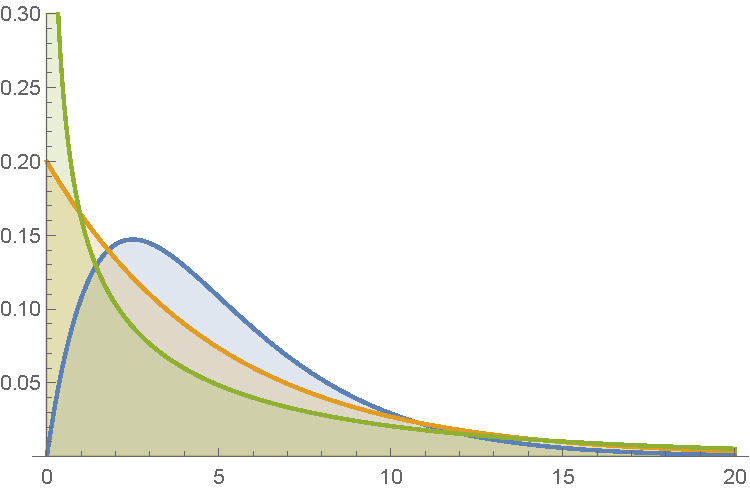
\includegraphics{gammadistrib.pdf}
\caption{Green: \(k=1/2\), Red: \(k=1\), Blue: \(k=2\)}
\end{figure}
\end{column}

\begin{column}{0.6\textwidth}
\begin{itemize}
\tightlist
\item
  In both groups, the infectious period is gamma distributed with mean
  \(1/\gamma\) and coefficient of variation \(1/\sqrt{k}\)
\item
  The gamma distribution is flexible in that it allows for heavily
  right-skewed distributions (i.e., \(k<1\)), and distributions with a
  central tendency (\(k>1\)).
\item
  Strongly right-skewed distributions (i.e., \(k<1\)) capture the
  property of there being a small proportion of individuals in the
  population with extremely long infectious period, who could therefore
  make many contacts leading to transmission over the course of being
  infected.
\end{itemize}
\end{column}
\end{columns}
\end{frame}

\begin{frame}{Mechanistic model is a finite mixture of negative
binomials}
\protect\hypertarget{mechanistic-model-is-a-finite-mixture-of-negative-binomials}{}
To find the probability distribution for the cumulative number of
transmission contacts generated by an infectious individual throughout
its entire infectious period the probability generating function is
given by \begin{align*}
    G_N(s) &= \int_0^{\infty} G(s,x) f_I(x) dx \notag \\ &= \int_0^\infty \left (p e^{\beta^S x (s-1)}+(1-p)e^{\beta x (s-1)} \right) \frac{(\gamma k)^k}{\Gamma(k)} x^{k-1}e^{-k \gamma x} dx.
\end{align*} Letting \(\beta /\gamma = R_0^R\) and
\(\beta^S /\gamma = R_0^S\), evaluating the integral yields
\begin{align*}
    G_N(s) &=  \frac{p}{(1 + \frac{\beta^S}{\gamma k}(1-s))^k} +   \frac{(1-p)}{(1 + \frac{\beta}{\gamma k}(1-s))^k} \notag \\&=  \frac{p}{(1 + \frac{R_0^S}{k}(1-s))^k} +   \frac{(1-p)}{(1 + \frac{R_0^R}{k}(1-s))^k}. 
\end{align*} This is a finite mixture of negative binomial models with
means \(R_0^R<R_0^S\) and dispersion parameter \(k\).
\end{frame}

\begin{frame}{Basic reproduction number for the mixture branching
process}
\protect\hypertarget{basic-reproduction-number-for-the-mixture-branching-process}{}
\begin{itemize}
\item
  The mean number of secondary infections per infectious individual per
  generation, is\\
  \begin{equation*}\label{eqn:R0}
   R_0= G_N'(1) = p\frac{ \beta^S }{\gamma } +(1-p)\frac{ \beta }  {\gamma  } = p R_0^S + (1-p) R_0^R.
  \end{equation*}
\item
  If \(R_0<1\) outbreaks are small and stutter to extinction; if
  \(R_0>1\) either the number of infectious individuals grows
  exponentially or outbreaks are minor and go extinct with probability
  \(s^*\) found by solving \(s=G_N(s)\).
\end{itemize}
\end{frame}

\begin{frame}{Probability mass function of mechanistic mixture model}
\protect\hypertarget{probability-mass-function-of-mechanistic-mixture-model}{}
Evaluating \(\frac{1}{j!} \frac{d^j}{ds^j} G_N(0) |_{s=0}\)
\(j=0,1,2\dots\) yields the probability mass function for the number of
secondary infections with parameters \(p\), \(k\), \(R_0^S\) and
\(R_0^R\), \scriptsize \begin{equation*}\label{eqn:nbinommixpmf}
    P(N=j) =  \frac{\Gamma(j+k)}{j! \Gamma (k)} \left [ p \left(\frac{k}{k+R_0^S} \right)^{k}\left (\frac{R_0^S}{k+R_0^S} \right )^j+ (1-p) \left(\frac{k}{k+R_0^R} \right)^{k}\left (\frac{R_0^R}{k+R_0^R} \right )^j \right ].
\end{equation*} \normalsize The model allows for a variety of infectious
histories including having extremely high risk of superspreading
transmission to others (e.g., high contact rate and long infectious
period), high risk of superspreading transmission to others (e.g., high
contact rate and fast recovery rate), moderate risk of being a
superspreader (e.g., low contact rate and long infectious period) and
being characterized by regular transmission (e.g., low contact rate and
fast recovery rate).
\end{frame}

\begin{frame}{Probability mass function of mechanistic model compared to
standard model}
\protect\hypertarget{probability-mass-function-of-mechanistic-model-compared-to-standard-model}{}
\includegraphics{Lab-meeting-presentation-Nov-21_files/figure-beamer/cars-1.pdf}
\end{frame}

\begin{frame}{Transmission chains (sizes of small outbreaks that go
extinct)}
\protect\hypertarget{transmission-chains-sizes-of-small-outbreaks-that-go-extinct}{}
We define a chain that goes extinct at time \(t\) by \[
Y = \sum_{i=0}^{t-1}x_i
\] with \(x_i\) denoting the cumulative number of offspring in the
\(i^{th}\) generation, and \(x_0 = 1\). The final size \(Y\) upon
extinction is a random variable with probability distribution
\(P(Y=y)\), \(y=1,2,...\).
\end{frame}

\begin{frame}{Deriving the chain size distribution}
\protect\hypertarget{deriving-the-chain-size-distribution}{}
To derive the chain size distribution for the Poisson mixture, we use
the result from Blumberg and Lloyd-Smith (2014) and therefore require
the derivatives of powers of the generating function. Let
\[T_y(z) = \frac{1}{y} (G_N(z))^y, \quad y = 1, 2, \dots \] Then the
probability of a chain having size \(y\) is
\begin{equation}\label{eqn:cluster}
    P(Y = y)  = \frac{1}{(y-1)!}T_y^{(y-1)}(z) \Bigr|_{z=0} 
\end{equation} To evaluate the derivatives of
\begin{equation}\label{eqn:Qy}
    (G_N(z))^y = \left (\frac{p}{(1 + \frac{R_0^S}{k}(1-s))^k} +   \frac{(1-p)}{(1 + \frac{R_0^R}{k}(1-s))^k} \right)^y,
\end{equation} we need to apply the chain rule for derivatives \(y-1\)
times.
\end{frame}

\begin{frame}{Derivation continued}
\protect\hypertarget{derivation-continued}{}
The \(n^{th}\) derivative of the inner function \(g_n\) of equation
\eqref{eqn:Qy}, \(n = 1, 2, \dots, y-1\), evaluated at \(z=0\) is
\scriptsize \begin{equation*}
    g_n^(n) =  p \frac{(R_0^S)^n}{k^{n-1}} \displaystyle \prod_{i=1}^{n-1} (k+i) \left(1+\frac{R_0^S}{k}\right)^{-k-n}+ (1-p)\frac{(R_0^R)^n}{k^{n-1}} \displaystyle \prod_{i=1}^{n-1} (k+i)\left (1+\frac{R_0^R}{k}\right)^{-k-n}.
\end{equation*} \normalsize The \(n^{th}\) derivative of the outer
function \(f_n\) of equation \eqref{eqn:Qy} evaluated at \(z=0\) is
\begin{equation*}
    f_n^(n) =  \frac{y!}{(y-n)! }\left (\frac{p}{(1 + \frac{R_0^S}{k})^k} +   \frac{(1-p)}{(1 + \frac{R_0^R}{k})^k} \right )^{y-n}, \quad n = 1, 2, \dots, y-1.
\end{equation*} The generalized chain rule (Faa di Bruno's formula)
yields \begin{equation}\label{eqn:bell}
  T_y^{(y-1)} \Bigr|_{z=0} = \sum_{n=1}^{y-1}  f_n B_{y,n}(g_1, g_2, \dots, g_{y-1-n})
\end{equation} where \(B_{y,n}\) are Bell polynomials of the \(g_n\).
\end{frame}

\begin{frame}{Chain size distribution of mechanistic model compared to
standard model}
\protect\hypertarget{chain-size-distribution-of-mechanistic-model-compared-to-standard-model}{}
\includegraphics{Lab-meeting-presentation-Nov-21_files/figure-beamer/unnamed-chunk-10-1.pdf}
\end{frame}

\begin{frame}{Statistics that show hallmarks of transmission
heterogeneity}
\protect\hypertarget{statistics-that-show-hallmarks-of-transmission-heterogeneity}{}
Hallmarks of heterogeneous transmission include:

\begin{itemize}
\item Greater variability in the number of secondary infections (fat tailed)
\item Smaller probability of major epidemics
\item Greater variability in chain sizes
\item Larger probability of observing no secondary infections and of observing small chains that go extinct
\end{itemize}
\end{frame}

\begin{frame}{Numerical study to compare mechanistic mixture model with
standard model}
\protect\hypertarget{numerical-study-to-compare-mechanistic-mixture-model-with-standard-model}{}
\begin{itemize}
\item
  Here we study the coefficient of variation of the number of secondary
  infections, the probability of a major outbreak, the probability of
  observing a small transmission chain of less than or equal to 10
  cases, and the coefficient of variation of small chain sizes
  (conditioned on extinction).
\item
  In each of the following, \(p\) and \(\delta\) are varied (which
  alters \(R_0^S\)) but
  \(R_0 = p R_0^S + (1-p) R_0^R= R_0^R + p \delta\) is fixed at
  \(R_0 =2\).
\end{itemize}
\end{frame}

\begin{frame}{Coefficient of variation of secondary infections}
\protect\hypertarget{coefficient-of-variation-of-secondary-infections}{}
\includegraphics{Lab-meeting-presentation-Nov-21_files/figure-beamer/unnamed-chunk-11-1.pdf}
\end{frame}

\begin{frame}{Probability of major outbreak}
\protect\hypertarget{probability-of-major-outbreak}{}
\includegraphics{Lab-meeting-presentation-Nov-21_files/figure-beamer/unnamed-chunk-12-1.pdf}
\end{frame}

\begin{frame}{Probability of observing a transmission chain of size
\(\leq\) 10}
\protect\hypertarget{probability-of-observing-a-transmission-chain-of-size-leq-10}{}
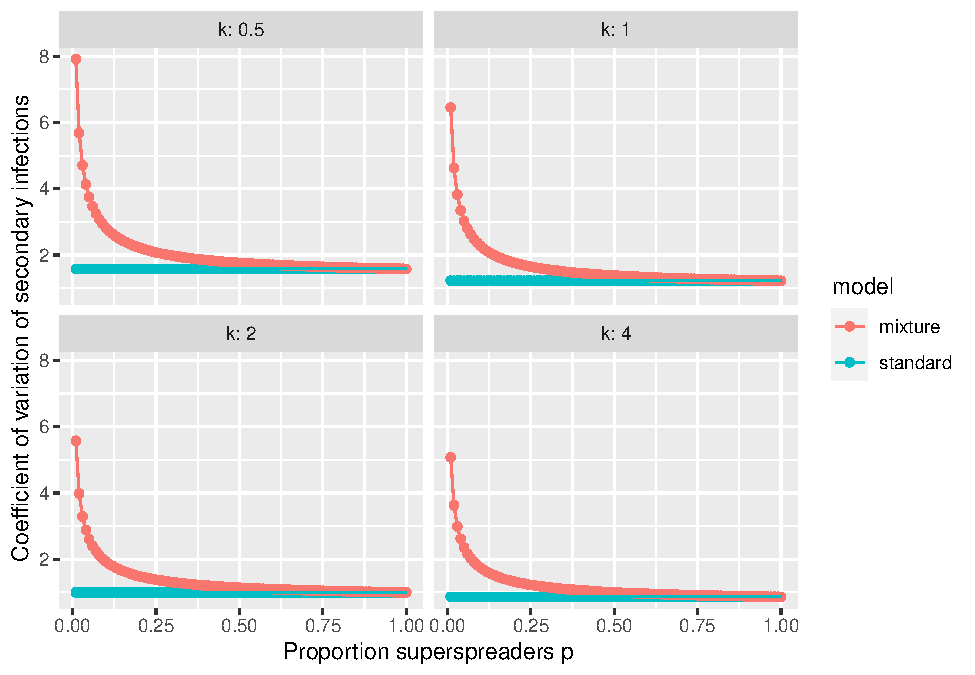
\includegraphics{Lab-meeting-presentation-Nov-21_files/figure-beamer/unnamed-chunk-13-1.pdf}
\end{frame}

\begin{frame}{Coefficient of variation of chain sizes}
\protect\hypertarget{coefficient-of-variation-of-chain-sizes}{}
\includegraphics{Lab-meeting-presentation-Nov-21_files/figure-beamer/unnamed-chunk-14-1.pdf}
\end{frame}

\begin{frame}{Preliminary conclusions from this study}
\protect\hypertarget{preliminary-conclusions-from-this-study}{}
\begin{itemize}
\item
  Having a small proportion of superspreaders with high \(R_0^S\) (i.e.,
  smaller values of \(p\) and larger values of \(\delta\)) lead to more
  heterogeneous epidemics than the standard model, even if the
  dispersion parameter \(k>1\).
\item
  Having a dispersion parameter \(k\) that is less than one is not
  necessary for the mixture model to exhibit hallmarks of superspreading
  transmission, suggesting that heterogeneity in the contact process is
  sufficient.
\end{itemize}
\end{frame}

\end{document}
